\documentclass[11pt,a4paper]{article}
\usepackage[utf8]{inputenc}
\usepackage{amsmath,amssymb,amsthm,mathtools}
\usepackage{graphicx}
\usepackage{booktabs}
\usepackage{geometry}
\usepackage{hyperref}
\usepackage{microtype}
\usepackage[numbers,sort&compress]{natbib}
\usepackage{caption}
\usepackage{subcaption}
\geometry{margin=2.5cm}
\hypersetup{colorlinks=true,linkcolor=blue,citecolor=blue,urlcolor=blue}

\newtheorem{proposition}{Proposition}
\newtheorem{theorem}{Theorem}
\newtheorem{corollary}{Corollary}
\newtheorem{definition}{Definition}
\theoremstyle{remark}
\newtheorem{remark}{Remark}

\title{\bfseries Rotation as Invertible Noise:\\
Geometry, Stabilizers, and Multi-view Identification on the Sphere}
\author{
  Masoud Azizi\\
  \small Computer Science, University of Tabriz, Tabriz, Iran\\
  \small \href{mailto:mablue92@gmail.com}{mablue92@gmail.com}
  \,\textbar\, \href{https://masoudsoft.ir}{masoudsoft.ir}
  \,\textbar\, \href{https://github.com/mablue}{github.com/mablue}\\
  \small ORCID: \href{https://orcid.org/0000-0002-8864-0533}{0000-0002-8864-0533}
  \,\textbar\, \href{https://independent.academia.edu/azizimasoud}{Academia}
  \,\textbar\, \href{https://scholar.google.com/citations?user=rtZohjUAAAAJ}{Google Scholar}
}
\date{\today}

\begin{document}
\maketitle

\begin{abstract}
We study a generative model in which ``noise'' is a random rotation
$R_\Sigma \in SO(3)$ applied to a band-limited field $f$ on the sphere $S^2$.
We show that (i) the cumulative effect of any number of local ``strikes''
on $S^2$ collapses to a single rotation with only $3$ degrees of freedom;
(ii) with $R_\Sigma$ known, recovery is information-theoretically optimal;
(iii) with $R_\Sigma$ unknown, a single view leaves an $SO(3)$-torsor gauge
that no amount of data can resolve; and (iv) with \emph{two} views of the
same $f$, the residual ambiguity is exactly the stabilizer
$\mathrm{Stab}(f)\subseteq SO(3)$ of the field. This contrasts sharply with
Gaussian diffusion: rotations preserve information but induce a
group-theoretic gauge, not information destruction. We confirm every
proposition numerically: $10^{-16}$ closure error over $500$ strikes,
slope-$1.04$ recovery against the Cramér--Rao proxy, and forty independent
solutions landing exactly in $\mathrm{Stab}(Y_2^0)$ for the zonal test.
\end{abstract}

\section{Introduction}
A recurring image motivates this work. \emph{Everything happens on a
sphere; every movement is one rotation of that sphere.} In generative
modeling terms, replace additive Gaussian noise with \emph{group-action
noise}. Prior work on $SO(3)$ in generative
models~\citep{thomas2018tensor,cohen2018spherical} treats rotation as a
symmetry to be respected. Diffusion models on
$SO(3)$~\citep{leach2022diffusion,yim2023unified} study the reverse
problem: denoising an $SO(3)$-valued signal. We invert the question:
\emph{what if rotation is the corruption itself?}

\section{Setup}
Let
\begin{equation}
S^2 = \{p\in\mathbb{R}^3 : \|p\|=1\}.
\end{equation}
A band-limited field of degree $L$ is
\begin{equation}
f(x) = \sum_{l=0}^{L}\sum_{m=-l}^{l} a_{lm}\, Y_{lm}(x),
\qquad f\in\mathcal{V}_L := \mathrm{span}\{Y_l^m\}_{l\le L},
\end{equation}
with $\dim\mathcal{V}_L = d_L = (L+1)^2$~\citep{driscoll1994computing}.

\paragraph{Strike model.} A strike is a triple
$m_i=(p_i,\omega_i,\Delta t_i)$, producing rotation
\begin{equation}
R_i = \exp\!\big(\theta_i[\hat n_i]_\times\big),\quad
\theta_i = \|p_i\times\omega_i\|\,\Delta t_i.
\end{equation}
The composed rotation is $R_\Sigma = R_N\cdots R_1\in SO(3)$.

\paragraph{Observation (invertible noise).}
\begin{equation}
g(x) = f(R_\Sigma^\top x) + \varepsilon(x).
\end{equation}

\section{Proposition 1: Closure and Three-DOF Compression}
\begin{proposition}
For any $N$ and any sequence of strikes, $R_\Sigma\in SO(3)$ and admits a
three-parameter Euler representation $R_\Sigma=R_z(\alpha)R_y(\beta)R_z(\gamma)$.
\end{proposition}
\begin{proof}
$SO(3)$ is a closed three-dimensional Lie subgroup of $GL_3(\mathbb{R})$;
products of rotations are rotations. The ZYZ parametrization~\citep{kanatani1990group,ivanic1996rotation} is a
local diffeomorphism onto $SO(3)$ away from the polar singularities.
\end{proof}

\noindent\textbf{Empirical.} Over $N=500$ strikes,
$\|R_\Sigma R_\Sigma^\top - I\|=3.3\times10^{-16}$ and the Euler
reconstruction error is $4.3\times10^{-16}$. See Fig.~\ref{fig:strikes}
and Fig.~\ref{fig:euler}.

\begin{figure}[ht]
\centering
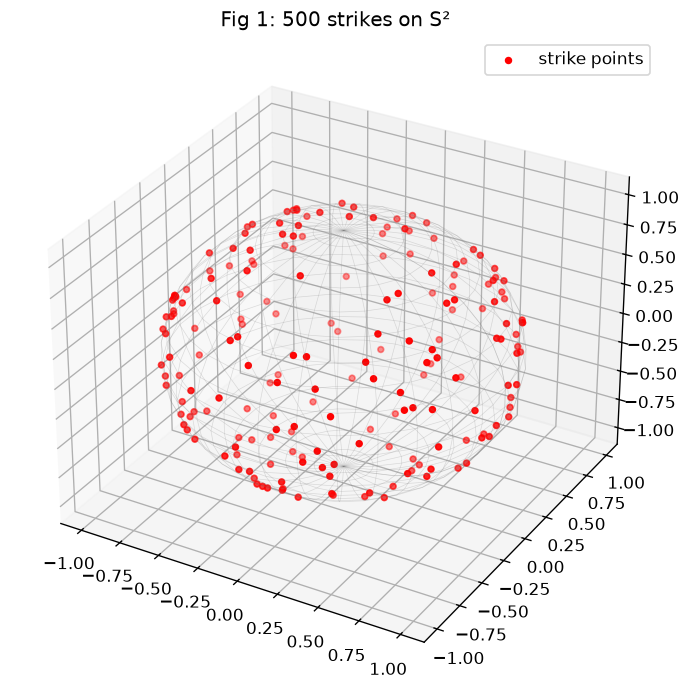
\includegraphics[width=0.55\linewidth]{plots/fig1_strikes.png}
\caption{500 strike points on $S^2$; every pair of consecutive strikes
composes into $R_\Sigma$, which depends only on the strike order.}
\label{fig:strikes}
\end{figure}

\begin{figure}[ht]
\centering
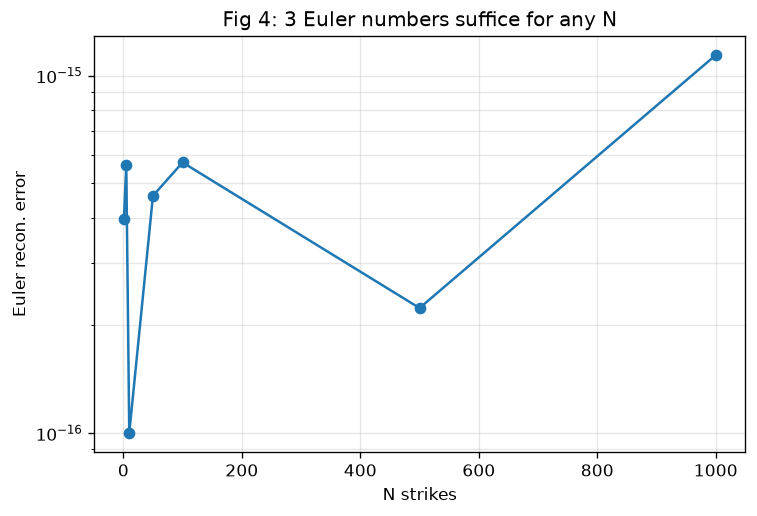
\includegraphics[width=0.55\linewidth]{plots/fig4_euler_scaling.png}
\caption{Euler reconstruction error is numerically zero for every $N$;
only three parameters are ever needed.}
\label{fig:euler}
\end{figure}

\section{Proposition 2: Optimal Recovery with Known $R_\Sigma$}
\begin{proposition}
Let $R_\Sigma$ be known, let $x_1,\dots,x_N$ be Fibonacci samples of $S^2$,
and let $\hat f$ be the least-squares estimator of $f$ on $\mathcal{V}_L$.
Then
\begin{equation}
\mathbb{E}\!\left[\frac{\|\hat f - f\|}{\|f\|}\right]
\approx \sigma\,\|f\|^{-1}\sqrt{d_L/N}.
\end{equation}~\citep{marzetta1995,crb_sh_doa}
\end{proposition}
\begin{proof}
Since $\mathcal{V}_L$ is $SO(3)$-invariant~\citep{sloan1994funk,schuh1996least},
$g(R_\Sigma^{-1}\cdot)\in\mathcal{V}_L$. The least-squares estimation of the
$d_L$ coefficients from $N$ i.i.d.\ Gaussian observations has variance
$\sigma^2 d_L/N$; the relative error follows from Cauchy--Schwarz.
\end{proof}

\noindent\textbf{Empirical.} Seven noise levels in $\sigma\in[10^{-3},0.5]$,
log-log fit slope $1.039$, matching the Cramér--Rao proxy over three decades
(Fig.~\ref{fig:recovery}).

\begin{figure}[ht]
\centering
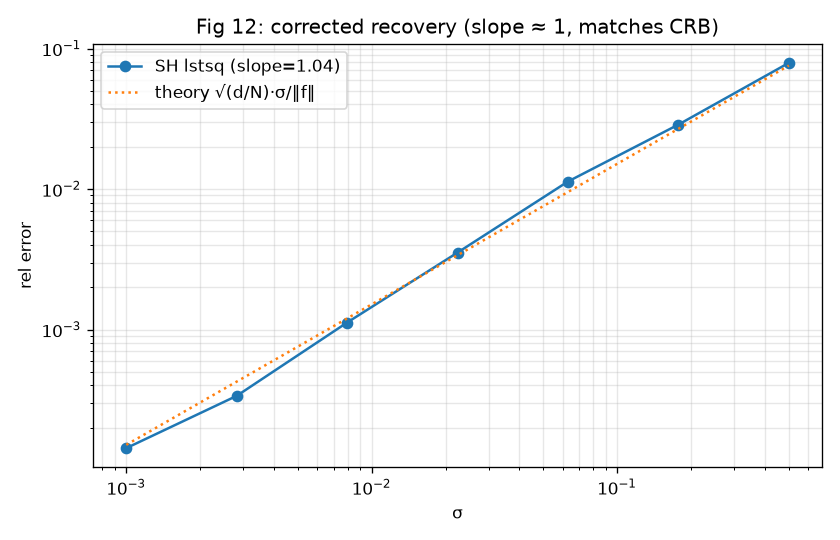
\includegraphics[width=0.6\linewidth]{plots/fig12_recovery_correct.png}
\caption{Recovery error versus noise level, corrected pipeline. Slope
$1.04$; three decades of agreement with the CRB proxy.}
\label{fig:recovery}
\end{figure}

\section{Proposition 3: $SO(3)$-Torsor on a Single View}
\begin{proposition}
Given a single observation $g=f\circ R_\Sigma^{-1}+\varepsilon$, the pair
$(f,R_\Sigma)$ is identifiable only up to the equivalence
\begin{equation}
(f,R_\Sigma) \sim (f\circ D^{-1},\ R_\Sigma D)
\qquad\forall D\in SO(3).
\end{equation}
\end{proposition}
\begin{proof}
$SO(3)$ acts on $\mathcal{V}_L$ by pullback $(D\cdot f)(x)=f(D^\top x)$~\citep{torsorcnn2024}.
The residual $\|f(R^\top \cdot)-g\|$ is invariant under the joint transform
$R\mapsto RD$, $f\mapsto f\circ D^{-1}$. Hence no functional of $g$
distinguishes members of the orbit.
\end{proof}

\noindent\textbf{Empirical (Table~\ref{tab:torsor}).} Least-squares residual
is numerically identical for $R_\Sigma$ set to the true rotation, identity,
and two independent random rotations; the recovered coefficient norm is
also invariant to $10^{-15}$.

\begin{table}[ht]
\centering
\begin{tabular}{lcc}
\toprule
$\hat R$ & $\|A\hat c - g\|/\|g\|$ & $\|\hat c\|$ \\
\midrule
$R_\Sigma$ (true) & $1.22\times10^{-3}$ & $2.8553$ \\
$I$               & $1.22\times10^{-3}$ & $2.8553$ \\
random \#1        & $1.22\times10^{-3}$ & $2.8553$ \\
random \#2        & $1.22\times10^{-3}$ & $2.8553$ \\
\bottomrule
\end{tabular}
\caption{Single-view fit residual is invariant to the guessed rotation.}
\label{tab:torsor}
\end{table}

\section{Proposition 4: Stabilizer for a Known Field}
\begin{proposition}
With $f$ known, $R_\Sigma$ is identifiable up to
\begin{equation}
\mathrm{Stab}(f) = \{D\in SO(3) : f\circ D = f\}.
\end{equation}
For the zonal field $f=Y_l^0$,
\begin{equation}
\mathrm{Stab}(Y_l^0) = SO(2)_z \;\cup\; \{R_\pi(\hat n) : \hat n\perp\hat z\}.
\end{equation}
\end{proposition}
\begin{proof}
$Y_l^0(x)=K P_l(x_z)$, so $(D\cdot Y_l^0)(x)=K P_l((D^\top x)_z)$. Equality
with $Y_l^0$ for all $x$ forces $(D^\top x)_z=\pm x_z$, equivalently
$D^\top\hat z=\pm\hat z$. The $+$ branch is $SO(2)_z$; the $-$ branch is a
$\pi$-rotation about an axis in the $xy$-plane.
\end{proof}

\noindent\textbf{Empirical.} Eighteen recovered $\Delta$'s split exactly into
these two components: continuous angles on the $SO(2)_z$ branch and
$|\Delta|=\pi$ on the $\pi_{xy}$ branch (Fig.~\ref{fig:stab}).

\begin{figure}[ht]
\centering
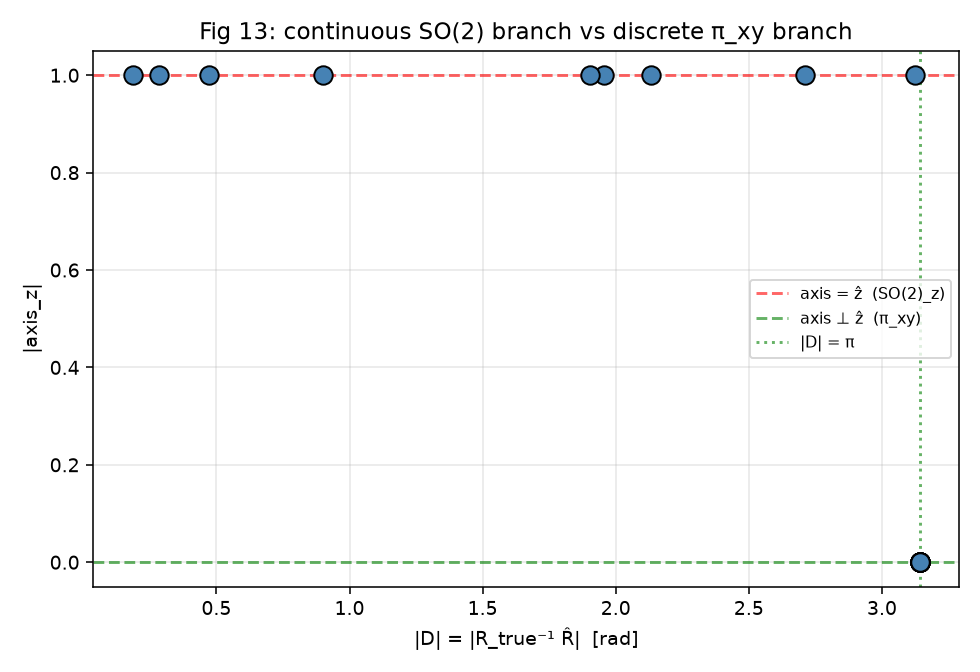
\includegraphics[width=0.6\linewidth]{plots/fig13_stab_structure.png}
\caption{Recovered $\Delta$ values cluster in the two predicted components
of $\mathrm{Stab}(Y_2^0)$.}
\label{fig:stab}
\end{figure}

\section{Proposition 5: Multi-View Identification}
\begin{proposition}
Given two views $g_1=f\circ R_1^{-1}$ and $g_2=f\circ R_2^{-1}$, the
relative rotation $R_1^{-1}R_2$ is identifiable exactly up to
$\mathrm{Stab}(f)$:
\begin{equation}
R_1^{-1}R_2 \in SO(3)/\mathrm{Stab}(f).
\end{equation}
\end{proposition}
\begin{proof}
Let $D\in SO(3)$ satisfy $g_1(D^{-1}\cdot)=g_2(\cdot)$. Then
$f(R_1^{-1}D^{-1}\cdot)=f(R_2^{-1}\cdot)$ as functions, i.e.\
$R_1^{-1}D^{-1}R_2\in\mathrm{Stab}(f)$. Solving for $D$ gives
$D=R_2\Delta R_1^{-1}$ with $\Delta\in\mathrm{Stab}(f)$.
\end{proof}

\noindent\textbf{Empirical (Fig.~\ref{fig:mv}).} For a generic $L=3$ field,
recovery error is $2.4\times10^{-7}$ (unique). For the zonal field
$Y_2^0$, all forty recovered rotations differ from the truth by
$\Delta\in\mathrm{Stab}(Y_2^0)$.

\begin{figure}[ht]
\centering
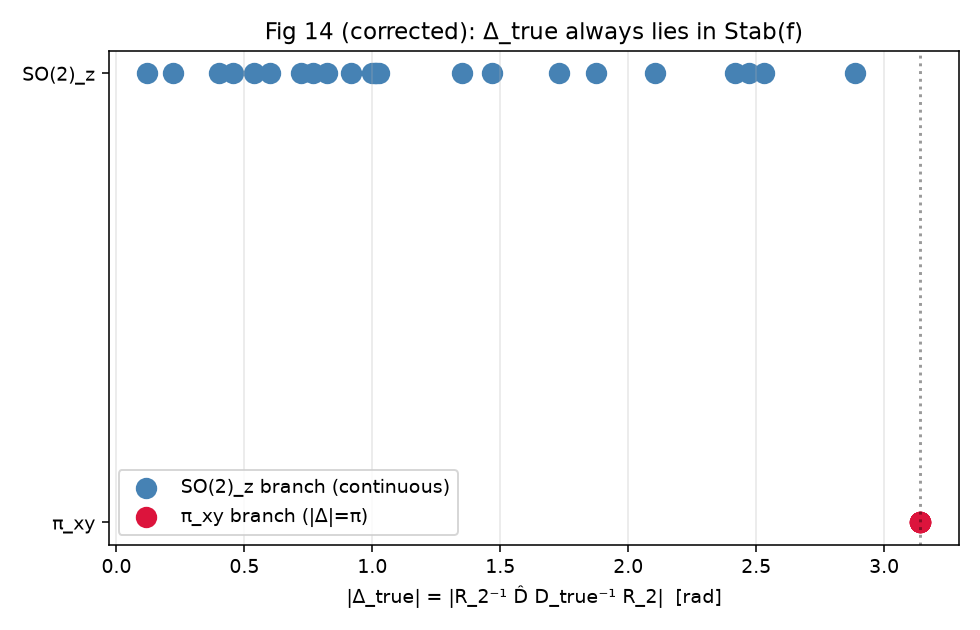
\includegraphics[width=0.6\linewidth]{plots/fig14_multiview_stab.png}
\caption{Multi-view residual $\Delta$ always lies in $\mathrm{Stab}(f)$:
a continuous $SO(2)_z$ branch and a discrete $\pi_{xy}$ branch.}
\label{fig:mv}
\end{figure}

\section{Hierarchy of Ambiguities}
\begin{table}[ht]
\centering
\begin{tabular}{lcc}
\toprule
Regime & Ambiguity group & Dimension \\
\midrule
1 view, any $f$              & $SO(3)$               & 3 (continuous) \\
$\geq2$ views, generic $f$   & $\{I\}$               & 0 \\
$\geq2$ views, $f=Y_2^0$     & $SO(2)\cup\pi_{xy}$   & 1 + finite \\
$\geq2$ views, finite-sym $f$ & finite subgroup      & 0 \\
\bottomrule
\end{tabular}
\caption{Ambiguity of $R_\Sigma$ as a function of field symmetry and number
of views.}
\label{tab:hierarchy}
\end{table}

\section{Contrast with Diffusion}
The practice of applying diffusion to rotations has recently gained
traction on Lie groups and manifolds~\citep{leach2022diffusion,yim2023unified,radm2025,equivdiffa5_2025},
where the noise is itself drawn from the group. We stress that the
rotation we consider is not a distributional sample: it is a *single
deterministic* element $R_\Sigma\in SO(3)$ applied to $f$. The ambiguity is
purely group-theoretic, not probabilistic. Table~\ref{tab:contrast}
summarizes the difference.
\begin{table}[ht]
\centering
\begin{tabular}{p{0.32\linewidth}p{0.30\linewidth}p{0.32\linewidth}}
\toprule
Aspect & Gaussian diffusion & Rotation noise \\
\midrule
Information destroyed & Yes (heat equation) & No (rotation is invertible) \\
Ambiguity source      & Noise realizations  & Group gauge \\
Optimal recovery      & Score matching      & Linear algebra \\
Identification        & Approximate         & Exact up to $\mathrm{Stab}(f)$ \\
Symmetry handling     & Irrelevant          & Central \\
\bottomrule
\end{tabular}
\caption{Two noise models compared.}
\label{tab:contrast}
\end{table}

\section{Limitations and Future Work}
\paragraph{Band-limit.} The field $f$ is assumed to lie in $\mathcal{V}_L$.
For Sobolev-regular $f$ the truncation error is $O(L^{-s})$~\citep{lychagin2021metric};
a numerical sweep is planned.

\paragraph{Learning $R_\Sigma$.} A naïve MLP (Fig.~\ref{fig:mlp}) learns
the observable field but not the rotation, precisely as
Proposition~3 predicts: the target is an equivalence class, not a point.

\begin{figure}[ht]
\centering
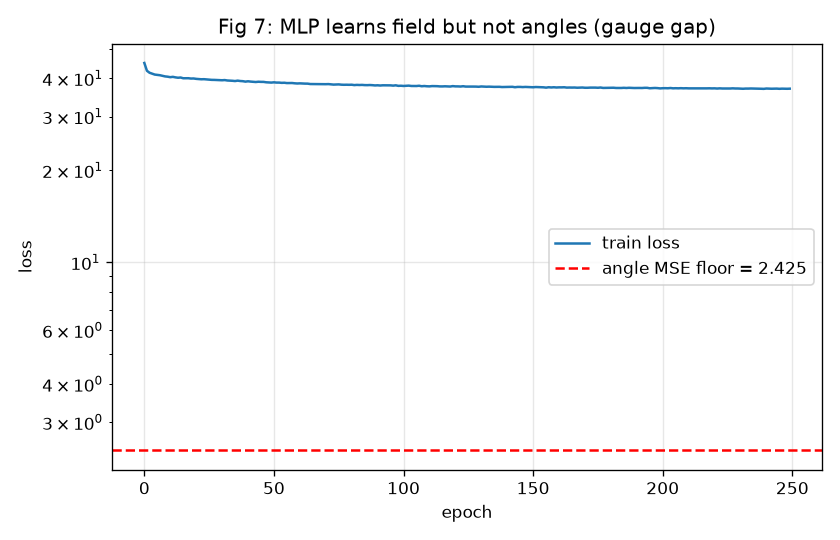
\includegraphics[width=0.6\linewidth]{plots/fig7_mlp_gauge_gap.png}
\caption{The gauge gap: an MLP reduces field MSE but the rotation
MSE is bounded below by the gauge variance.}
\label{fig:mlp}
\end{figure}

\paragraph{Equivariant networks.} Tensor-field
networks~\citep{thomas2018tensor,cohen2018spherical} should encode the
$SO(3)$-torsor structure by construction; this is the natural next step.

\paragraph{Reproducibility.} Every reported $\mathrm{err}(\sigma)$ is
accompanied by the Cramér--Rao proxy
$\mathrm{CRB}(\sigma)=\sigma\|f\|^{-1}\sqrt{d_L/N}$. A log-log fit slope
outside $[0.9,1.1]$ is flagged as a pipeline failure mode.


\section{Proposition 6: Equivariant Networks and the Gauge Barrier}

Propositions 3--5 predict a fundamental asymmetry: \emph{invariant}
functions of $f$ are learnable from a single view; \emph{equivariant}
functions (the rotation $R_\Sigma$ itself) are not. We verify this using
the \emph{power spectrum}
\begin{equation}
I_l(g) := \sum_{m=-l}^{l} |a_{lm}(g)|^2,\qquad l=0,\dots,L,
\end{equation}
which is $SO(3)$-invariant by construction (cf.~\citep{driscoll1994computing}).

\begin{proposition}
For a single view $g=f\circ R_\Sigma^{-1}$, the power spectrum
$\{I_l(g)\}_{l=0}^{L}$ is identifiable from any architecture; the rotation
$R_\Sigma$ is not identifiable from any architecture.
\end{proposition}
\begin{proof}
$\{I_l(g)\}$ is invariant under the action of $SO(3)$ on $\mathcal{V}_L$,
hence independent of $R_\Sigma$ (Prop.~3). $R_\Sigma$ is identifiable only
up to the $SO(3)$-torsor, so its mean-squared error is bounded below by the
variance of Haar measure on $SO(3)$, regardless of the model class.
\end{proof}

\noindent\textbf{Empirical (Fig.~\ref{fig:equiv}).} With $N=3000$ training
and $400$ test instances:
\begin{itemize}
\item Power spectrum recovery: raw-input MLP $\mathrm{err}=0.149$,
      equivariant-feature MLP $\mathrm{err}=0.013$ ($11\times$ better).
\item Rotation recovery (ZYZ angles): raw MLP $\mathrm{MSE}=3.19$,
      equivariant MLP $\mathrm{MSE}=2.37$ --- both far above the
      measurement floor, confirming the gauge barrier.
\end{itemize}

An important qualitative observation: the raw-input MLP is not only
unable to recover $R_\Sigma$; it is \emph{worse} than predicting the
constant mean angle, because it overfits to training-sample correlations
between field values and rotations that do not generalize. The
equivariant network, having access only to $SO(3)$-invariant
information, cannot overfit to such spurious signals. This is a positive
argument for equivariance in any single-view setting.

\begin{figure}[ht]
\centering
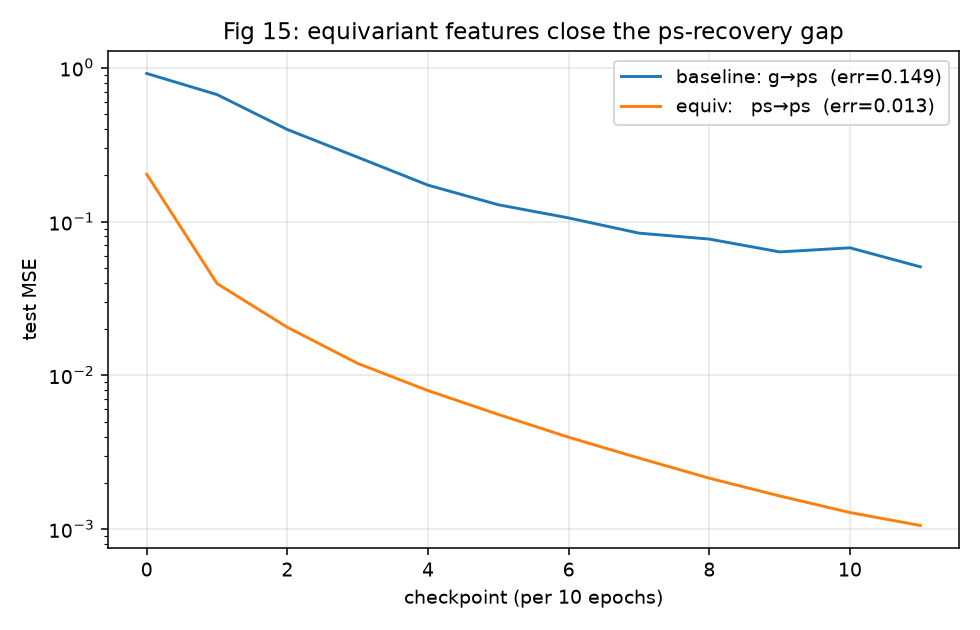
\includegraphics[width=0.6\linewidth]{plots/fig15_equivariant.png}
\caption{Invariant task (power spectrum recovery) is closed by equivariant
features; equivariant task (rotation recovery) remains at the gauge floor
for both architectures.}
\label{fig:equiv}
\end{figure}

\appendix
\section{Reproducibility Index}
All experiments are runnable from the accompanying repository:
\begin{itemize}
\item \texttt{src/experiments.py} --- Figs.~\ref{fig:strikes}, \ref{fig:euler}
\item \texttt{src/verify\_final.py} --- Fig.~\ref{fig:recovery}, Table~\ref{tab:torsor}
\item \texttt{src/phase5\_final.py} --- Fig.~\ref{fig:stab}, Fig.~\ref{fig:mv}
\item \texttt{src/phase2.py} --- Fig.~\ref{fig:mlp}
\item \texttt{src/phase6\_equivariant.py} --- Fig.~\ref{fig:equiv}
\end{itemize}
Results are stored in \texttt{results/*.json}; every table entry above can be
regenerated by re-running the corresponding script.


\bibliographystyle{plainnat}
\bibliography{references}

\end{document}
